\documentclass[12pt]{article}
\usepackage[utf8]{inputenc}
\usepackage{float}
\usepackage{amsmath}


\usepackage[hmargin=3cm,vmargin=6.0cm]{geometry}
%\topmargin=0cm
\topmargin=-2cm
\addtolength{\textheight}{6.5cm}
\addtolength{\textwidth}{2.0cm}
%\setlength{\leftmargin}{-5cm}
\setlength{\oddsidemargin}{0.0cm}
\setlength{\evensidemargin}{0.0cm}

%misc libraries goes here
\usepackage{tikz}
\usetikzlibrary{automata,positioning}

\begin{document}

\section*{Student Information } 
%Write your full name and id number between the colon and newline
%Put one empty space character after colon and before newline
Full Name :  Nazır Bilal Yavuz\\
Id Number :  2099471\\

% Write your answers below the section tags
\section*{Answer 1}

\subsection*{a.}

$S \rightarrow aSXaX$  ------ (R1) \\
$S \rightarrow bSXbX$  ------ (R2) \\
$S \rightarrow c$  ------ (R3) \\ 
$X \rightarrow aX$  ------ (R4) \\
$X \rightarrow bX$  ------ (R5) \\
$X \rightarrow e$  ------ (R6) \\
\\
$(p,a,e),(p,a)$ for each $a \in \sum$  ------ ($\bigtriangleup1$)\\\\
$(p,e,XaXSa),(p,S)$  ------ ($\bigtriangleup2$)\\\\
$(p,e,XbXSb),(p,S)$  ------ ($\bigtriangleup3$)\\\\
$(p,e,c),(p,S)$  ------ ($\bigtriangleup4$)\\\\
$(p,e,Xa),(p,X)$  ------ ($\bigtriangleup5$)\\\\
$(p,e,Xb),(p,X)$  ------ ($\bigtriangleup6$)\\\\
$(p,e,e),(p,X)$  ------ ($\bigtriangleup7$)\\\\
$(p,e,S),(p,e)$  ------ ($\bigtriangleup8$)\\\\

\subsection*{b.}
\begin{table}[H]
\centering
\caption{Tracing abbcbabbaa}
\label{my-label}
\begin{tabular}{|l|l|l|l|l|}
\hline
Step & State & Unread Input & Stack    & Transition Used \\ \hline
0    & p     & abbcbabbaa   & empty    &                \\ \hline
1    & p     & bbcbabbaa    & a        & 1               \\ \hline
2    & p     & bcbabbaa     & ba       & 1               \\ \hline
3    & p     & cbabbaa      & bba      & 1               \\ \hline
4    & p     & babbaa       & cbba     & 1               \\ \hline
5    & p     & babbaa       & Sbba     & 4               \\ \hline
6    & p     & babbaa       & XSbba    & 7               \\ \hline
7    & p     & abbaa        & bXSbba   & 1               \\ \hline
8    & p     & bbaa         & abXSbba  & 1               \\ \hline
9    & p     & bbaa         & XabXSbba & 7               \\ \hline
10   & p     & bbaa         & XbXSbba  & 5               \\ \hline
11   & p     & bbaa         & Sba      & 3               \\ \hline
12   & p     & bbaa         & XSba     & 7               \\ \hline
13   & p     & baa          & bXSba    & 1               \\ \hline
14   & p     & aa           & bbXSba   & 1               \\ \hline
15   & p     & aa           & XbbXSba  & 7               \\ \hline
16   & p     & aa           & XbXSba   & 6               \\ \hline
17   & p     & aa           & Sa       & 3               \\ \hline
18   & p     & aa           & XSa      & 7               \\ \hline
19   & p     & a            & aXSa     & 1               \\ \hline
20   & p     & empty        & aaXSa    & 1               \\ \hline
21   & p     & empty        & XaaXSa   & 7               \\ \hline
22   & p     & empty        & XaXSa    & 5               \\ \hline
23   & p     & empty        & S        & 2               \\ \hline
24   & p     & empty        & empty    & 8                \\ \hline
\end{tabular}
\end{table}


\section*{Answer 2}

\subsection*{a.}
We can define the Turing Machine which computes $f(x)$ as $M = (K,\Sigma,\delta, s, H)$, where
$K = \{s,e_0,o_0,e_1,e_2,e_3,o_1,o_2$, $\Sigma = \{\sqcup,1,\triangleright\}$, $H = \{h_1\}
$ and the transition function is defined as follows;

\begin{align*}
&\delta_1(s,\sqcup) = (e_0,\sqcup,\rightarrow) \\\\
&\delta_1(o_0,1) = (e_0,x,\rightarrow) && &\delta_1(e_0,1) = (o_0,x,\rightarrow) \\
&\delta_1(o_0,\sqcup) = (o_1,\sqcup,\leftarrow) && &\delta_1(e_0,\sqcup) = (e_1,\sqcup,\leftarrow) \\
&\delta_1(o_1,x) = (o_1,x,\leftarrow) && &\delta_1(e_1,x) = (e_1,x,\leftarrow) \\
&\delta_1(o_1,\sqcup) = (o_2,\sqcup,\rightarrow) && &\delta_1(e_1,\sqcup) = (e_2,\sqcup,\rightarrow)\\
&\delta_1(o_2,x) = (o_2,1,\rightarrow) && &\delta_1(e_2,x) = (e_3,1,\rightarrow) \\
&\delta_1(o_2,\sqcup) = (h_1,1,\rightarrow) && &\delta_1(e_3,x) = (e_3,x,\rightarrow) \\
& &&  &\delta_1(e_3,\sqcup) = (e_4,\sqcup,\leftarrow) \\
& &&  &\delta_1(e_4,x) = (e_5,\sqcup,\leftarrow) \\
& &&  &\delta_1(e_5,x) = (e_5,x,\leftarrow) \\
& &&  &\delta_1(e_5,1) = (e_3,1,\rightarrow) \\
& &&  &\delta_1(e_3,\sqcup) = (h_1,\sqcup,\rightarrow)
\end{align*}
\\
In this TM first go 1 from $\sqcup$ and check that it is even or odd while checking fill tape with $x$. \\\\
If it is odd go to the first $x$ and make all $x$ 1 and when you see $\sqcup$ make it 1 too. \\
This means $f(x) = x + 1$\\\\
If it is odd go to the first $x$ make it 1 and go right until find $\sqcup$ .\\
When you find $\sqcup$ go one left which is righmost $x$.
After that, make this $x$ to 1.\\
After that go leftmost $x$ and make it 1.\\
Follow this pattern...\\
This means $f(x) = x / 2$


\section*{Answer 3}

If we can not go to the left of the Turing Machine that is not completely Turing Machine. We can not use full capability of Turing Machine so that this type of Turing Machine looks like DFA more than Turing Machine. This type of Turing Machines accept regular languages.


\section*{Answer 4}





\subsection*{a.}

We can define the Queue Based Turing Machine which computes\\
 $f(x)$ as $M = (K,\Sigma,\delta, \top, \heartsuit, \clubsuit,\wp,\aleph, s,b, H)$, where;\\
\\
$K=$ set of states\\
$\Sigma=$ input alphabet not containing $(\sqcup, \top,\clubsuit)$\\
$\delta=$ transition function\\
$\top=$ tape alphabet\\
$\heartsuit=$ queue symbol for at the start set rear and front \\
$\clubsuit=$ rear symbol\\
$\wp=$ front symbol\\
$\aleph=$ between left of head and right of head(explanation is in part d)\\
$s=$ starting state, must be in $K$\\
$b=$ blank symbol, must be in $\top$\\
$H=$ set of final states 

\subsection*{b.}

Queue Based Turing Machine configuration is $(q, w, u)$. \\
The current state is $q$.\\
$w$ is the which $\wp_{(front symbol)}$ shows.\\
$u$ is the which $\clubsuit_{(rear symbol)}$ shows.\\

\subsection*{c.}



\subsection*{d.}

In Queue based TM, front shows head of standard TM.\\
After that right of head comes.\\
After that $\aleph$.\\
After that left of head comes.\\
For example $abc$ $d_{head}$ $ef$ is in Queue based TM equals to $def$ $\aleph$ $abc$\\\\
To make $d \rightarrow x, R$ dequeue front and enqueue x. After that dequeue front and enqueue symbol which is dequeued. At final state it looks like $ef$ $\aleph$ $abcx$.\\
To make $d \leftarrow x, R$ dequeue front and enqueue x. After that dequeue front and enqueue symbol which is dequeued. At final state it looks like $cxef$ $\aleph$ $ab$.\\\\
To access the rear element in the queue-based TM we can make $d \leftarrow d, L$\\
Front element in the queue-based TM is head of standard TM.

\subsection*{e.}




\section*{Answer 5}

\subsection*{a.}


\begin{center}
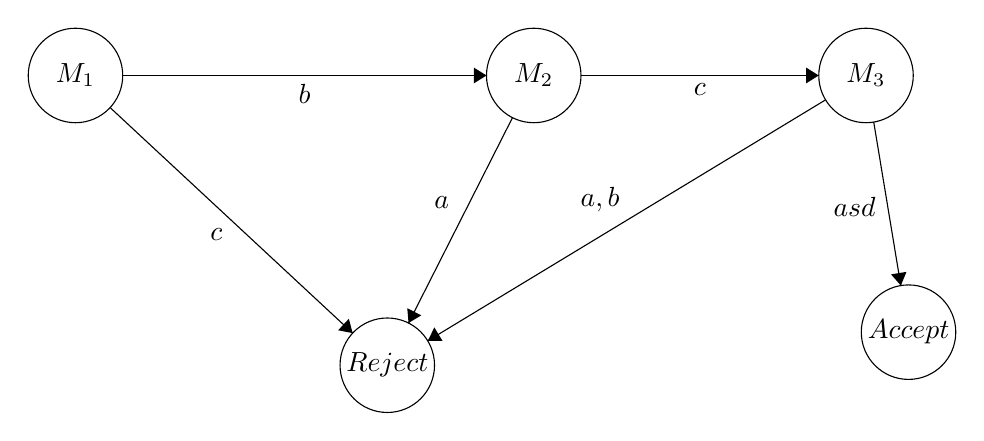
\begin{tikzpicture}[scale=0.2]
\tikzstyle{every node}+=[inner sep=0pt]
\draw [black] (15.1,-22.7) circle (3);
\draw (15.1,-22.7) node {$M_1$};
\draw [black] (44.2,-22.7) circle (3);
\draw (44.2,-22.7) node {$M_2$};
\draw [black] (65.3,-22.7) circle (3);
\draw (65.3,-22.7) node {$M_3$};
\draw [black] (34.9,-41.1) circle (3);
\draw (34.9,-41.1) node {$Reject$};
\draw [black] (68,-39) circle (3);
\draw (68,-39) node {$Accept$};
\draw [black] (18.1,-22.7) -- (41.2,-22.7);
\fill [black] (41.2,-22.7) -- (40.4,-22.2) -- (40.4,-23.2);
\draw (29.65,-23.2) node [below] {$b$};
\draw [black] (47.2,-22.7) -- (62.3,-22.7);
\fill [black] (62.3,-22.7) -- (61.5,-22.2) -- (61.5,-23.2);
\draw (54.75,-23.2) node [below] {$c$};
\draw [black] (17.3,-24.74) -- (32.7,-39.06);
\fill [black] (32.7,-39.06) -- (32.46,-38.15) -- (31.78,-38.88);
\draw (24.04,-32.39) node [below] {$c$};
\draw [black] (42.85,-25.38) -- (36.25,-38.42);
\fill [black] (36.25,-38.42) -- (37.06,-37.93) -- (36.17,-37.48);
\draw (38.86,-30.78) node [left] {$a$};
\draw [black] (62.73,-24.25) -- (37.47,-39.55);
\fill [black] (37.47,-39.55) -- (38.41,-39.56) -- (37.89,-38.7);
\draw (48.41,-31.4) node [above] {$a,b$};
\draw [black] (65.79,-25.66) -- (67.51,-36.04);
\fill [black] (67.51,-36.04) -- (67.87,-35.17) -- (66.89,-35.33);
\draw (65.94,-31.07) node [left] {$asd$};
\end{tikzpicture}
\end{center}


$M_1, M_2, M_3$ are TMs.\\
$M_1$ is for $a^n$\\
$M_2$ is for $b^{2^n}$.\\
$M_3$ is for $c^{3n}$.\\



\subsection*{b.}



\section*{Answer 6}

\subsection*{a.}

Yes, there exist $M_1, M_2, M_3, M_4, M_5$ which represents $L_1, L_2, L_3, L_4, L_5$ respectively.

\subsection*{b.}

\subsection*{c.}

\subsection*{d.}


%Do not submit solutions for Question 7, yet do solve it.


\end{document}

​

